\section{Weights analysis} \label{chap:weight:analysis}

    Most machine learning algorithm are primarily used as black box approaches~\cite{ribeiro2016should}. % explainability
    It is hard, to justify their predictions or to extract some insight from them. 
    
    We designed eLSA with interpretability in mind.
    Because eLSA just re-weights words, we argue that it is more easily interpretable and we can extract important insight about our data from it.
    In this section, we present such insight.
    
    \subsection{Effect of reweighting}
    The core of our approach it to reweight the co-occurrence matrix $M$ with weights $w'$. 
    These weights effectively change importance of some words with regards to the classification task.
    We can directly examine them and see, what words were boosted and what words were inhibited.
    
    Note that high word importance still does not tell us anything about the label. 
    We do not know (at least not from $w'$ alone), if the word is important for positive ($1$,~positive sentiment) or negative label ($0$, negative sentiment).
    
    Values in $w'$ tell us which words are underweighted by the original weighting schemes and which are overweighted.
    We examine mostly the CR dataset and the TREC-DESC dataset, as eLSA shows some interesting insights particularly into these two datasets.

    \subsubsection{Most reweighted words}
    
    First, we examine the words that our approach reweighted the most (most extreme $w'$).
    We present the $10$ most originally underweighted and the $10$ most originally overweighted words for combinations of CR and TREC-DESC datasets and weighting schemes \texttt{None} (no scheme was used), \texttt{tfidf} (basic unsupervised scheme) and \texttt{tfig} (supervised scheme).
    

\begin{table}[H]
    \centering
    \begin{minipage}{.4\linewidth}
      \centering
        \begin{tabular}{lr}
\toprule
    words &  $w'$ \\
\midrule
     slow &  3.06 \\
    happy &  2.65 \\
      you &  2.60 \\
    works &  2.51 \\
     good &  2.50 \\
      bad &  2.46 \\
      and &  2.45 \\
   expect &  2.38 \\
 pictures &  2.38 \\
   highly &  2.34 \\
\bottomrule
\end{tabular}

      \subcaption{Words with highest $w'$}
    \end{minipage}
    \begin{minipage}{.4\linewidth}
      \centering
        \begin{tabular}{lr}
\toprule
  words &  $w'$ \\
\midrule
   that &  0.25 \\
     am &  0.23 \\
   down &  0.22 \\
    two &  0.21 \\
   then &  0.21 \\
      3 &  0.20 \\
   give &  0.15 \\
     is &  0.14 \\
      n &  0.07 \\
 diaper &  0.02 \\
\bottomrule
\end{tabular}

      \subcaption{Words with lowest $w'$}
    \end{minipage} 
    \caption{Most reweighted words on CR dataset for scheme None}
    \label{tab:words:CR:None}
\end{table}

    In table~\ref{tab:words:CR:None} we see that if we use weighting scheme \texttt{None} (term vector), 
    we underweight some words that are obviously important such as \texttt{good} and \texttt{bad}.
    Our approach can correctly identify these words and boost their weights.
    In the same time, our approach can inhibit unrelated words like: \texttt{is}, \texttt{am}, or \texttt{that}.
    We see that using this weighting scheme (not using weighting scheme at all) is definitely not locally optimal.
    
    
\begin{table}[h]
    \centering
    \begin{minipage}{.4\linewidth}
      \centering
        \begin{tabular}{lr}
\toprule
 words &  $w'$ \\
\midrule
   not &  3.25 \\
 price &  2.92 \\
  good &  2.57 \\
  love &  2.40 \\
    if &  2.34 \\
 would &  2.21 \\
 worst &  2.08 \\
 works &  2.08 \\
    to &  2.07 \\
     i &  2.01 \\
\bottomrule
\end{tabular}

      \subcaption{Words with highest $w'$}
    \end{minipage}
    \begin{minipage}{.4\linewidth}
      \centering
        \begin{tabular}{lr}
\toprule
    words &  $w'$ \\
\midrule
    light &  0.18 \\
 problems &  0.17 \\
   camera &  0.11 \\
      few &  0.10 \\
    their &  0.08 \\
  quality &  0.06 \\
  battery &  0.01 \\
        a &  0.00 \\
        n &  0.00 \\
       be &  0.00 \\
\bottomrule
\end{tabular}
      \subcaption{Words with lowest $w'$}
    \end{minipage} 
    \caption{Most reweighted words on CR dataset for scheme tfidf}
    \label{tab:words:CR:tfidf}
\end{table}

    In table~\ref{tab:words:CR:tfidf} we display results for \texttt{tfidf}. 
    Recall from section~\ref{sec:term:weights} that \texttt{tfidf} decreases importance of words that are common in the dataset.
    However, we see (and already know) that such words may be very important for the classification task.
    This is exactly what eLSA can find out. 
    Our approach boosted words like \texttt{good} and \texttt{worst} that are very common and very discriminative.
    Moreover, our approach boosted the word \texttt{not} that is usually completely removed from the datasets, because it is considered to be a stop word. 
    Last, but not least, eLSA almost completely inhibited the preposition \texttt{a}~that almost certainly does not hold any importance for any classification task.


\begin{table}[H]
    \centering
    \begin{minipage}{.4\linewidth}
      \centering
        \begin{tabular}{lr}
\toprule
    words &  $w'$ \\
\midrule
 features &  3.33 \\
 symantec &  3.05 \\
  perfect &  2.96 \\
      the &  2.94 \\
     flaw &  2.87 \\
      bit &  2.83 \\
     slow &  2.71 \\
  awesome &  2.69 \\
  process &  2.66 \\
  useless &  2.64 \\
\bottomrule
\end{tabular}

      \subcaption{Words with highest $w'$}
    \end{minipage}
    \begin{minipage}{.4\linewidth}
      \centering
        \begin{tabular}{lr}
\toprule
  words &  $w'$ \\
\midrule
   that &  0.92 \\
     is &  0.88 \\
  great &  0.83 \\
     't &  0.83 \\
    not &  0.72 \\
   very &  0.62 \\
      , &  0.59 \\
    and &  0.52 \\
 camera &  0.43 \\
   this &  0.25 \\
\bottomrule
\end{tabular}

      \subcaption{Words with lowest $w'$}
    \end{minipage} 
    \caption{Most reweighted words on CR dataset for scheme tfig}
    \label{tab:words:CR:tfig}
\end{table}

    In table~\ref{tab:words:CR:tfig}, we see results for a supervised weighting scheme \texttt{tfig}.
    When we look at the table b, we see that only a few fords were really overweighted by the scheme. 
    For some reason, words: \texttt{this}, \texttt{,}, \texttt{and} have high weights and our approach identified them as not important.
    We see that other words are not penalized very much ($0.8$ or $0.9$).
    On the other hand, it looks like this scheme undervalues some rather interesting words like \texttt{awesome} or \texttt{slow}.
    Interesting is a word \texttt{the}, what is always considered to be a stop word and is usually removed. 
    However, according to our approach, it is underweighted. 
    We think that it is because it can signify some form of superlative and hence indicate sentiment polarity.
    

    Now we look at the TREC-DESC dataset. 
    Recall from section~\ref{sec:data:overview} that in this task we have some question, and we need to predict, whether the answer to this question is a some form of a description (in contrary to some numerical answer for example).
    
    
    

\begin{table}[H]
    \centering
    \begin{minipage}{.4\linewidth}
      \centering
        \begin{tabular}{lr}
\toprule
  words &   $w'$ \\
\midrule
   what &  13.20 \\
     is &   9.89 \\
    how &   8.39 \\
    are &   5.08 \\
   mean &   4.86 \\
   long &   4.60 \\
    why &   3.96 \\
    big &   3.93 \\
 reason &   2.95 \\
 origin &   2.89 \\
\bottomrule
\end{tabular}

      \subcaption{Words with highest $w'$}
    \end{minipage}
    \begin{minipage}{.4\linewidth}
      \centering
        \begin{tabular}{lr}
\toprule
    words &  $w'$ \\
\midrule
     form &  0.57 \\
     name &  0.55 \\
    where &  0.52 \\
 language &  0.51 \\
     does &  0.48 \\
       of &  0.46 \\
     when &  0.45 \\
      and &  0.20 \\
      the &  0.15 \\
        , &  0.07 \\
\bottomrule
\end{tabular}

      \subcaption{Words with lowest $w'$}
    \end{minipage} 
    \caption{Most reweighted words on DESC dataset for scheme None}
    \label{tab:words:TREC:none}
\end{table}

    If we use just the term vectors (scheme \texttt{None}), there are again typical words that we underweight.
    The answer obviously depends on the interrogative pronoun such as: \texttt{who} or \texttt{what}.
    Also, words like \texttt{origin}, \texttt{mean}, and \texttt{reason} probably associate with some desired explanation.
    On the other hand, words like \texttt{does}, \texttt{of}, and \texttt{and} were identified like not important.
    We also see interesting decrease for words like \texttt{when} and \texttt{where}.
    We hypothesize that even though these words are interrogative pronouns, they are usually used to form dependent clauses that do not tell anything about the type of the desired answer.
    Our approach even correctly inhibited the token \texttt{,}.
 

\begin{table}[h]
    \centering
    \begin{minipage}{.4\linewidth}
      \centering
        \begin{tabular}{lr}
\toprule
words &  $w'$ \\
\midrule
   is &  6.25 \\
  how &  5.87 \\
 what &  3.73 \\
   in &  3.60 \\
 mean &  3.51 \\
   of &  3.10 \\
 come &  3.09 \\
 long &  2.96 \\
  for &  2.94 \\
  the &  2.39 \\
\bottomrule
\end{tabular}

      \subcaption{Words with highest $w'$}
    \end{minipage}
    \begin{minipage}{.4\linewidth}
      \centering
        \begin{tabular}{lr}
\toprule
        words &  $w'$ \\
\midrule
         from &  0.42 \\
          its &  0.41 \\
     nickname &  0.38 \\
      address &  0.34 \\
 abbreviation &  0.32 \\
         fast &  0.32 \\
         term &  0.25 \\
         word &  0.24 \\
      between &  0.04 \\
            ? &  0.00 \\
\bottomrule
\end{tabular}

      \subcaption{Words with lowest $w'$}
    \end{minipage} 
    \caption{Most reweighted words on DESC dataset for scheme tfidf}
    \label{tab:words:trec:tfidf}
\end{table}

    Because we know that interrogative pronouns are important and abundant, we know that \texttt{tfidf} will underweight them.
    eLSA correctly compensated weight of these words.
    
    

\begin{table}[H]
    \centering
    \begin{minipage}{.4\linewidth}
      \centering
        \begin{tabular}{lr}
\toprule
      words &  $w'$ \\
\midrule
         is &  7.69 \\
        are &  4.52 \\
       what &  3.52 \\
       mean &  3.44 \\
     origin &  3.42 \\
 difference &  3.20 \\
       much &  2.91 \\
       long &  2.79 \\
      where &  2.72 \\
 definition &  2.71 \\
\bottomrule
\end{tabular}

      \subcaption{Words with highest $w'$}
    \end{minipage}
    \begin{minipage}{.4\linewidth}
      \centering
        \begin{tabular}{lr}
\toprule
words &  $w'$ \\
\midrule
  out &  1.00 \\
 name &  0.98 \\
  you &  0.97 \\
 does &  0.93 \\
   in &  0.90 \\
  who &  0.83 \\
   do &  0.71 \\
    ? &  0.59 \\
  was &  0.46 \\
  the &  0.00 \\
\bottomrule
\end{tabular}

      \subcaption{Words with lowest $w'$}
    \end{minipage} 
    \caption{Most reweighted words on DESC dataset for scheme tfig}
    \label{tab:words:TREC:tfig}
\end{table}

    In table~\ref{tab:words:TREC:tfig} we see that even supervised weighting scheme \texttt{tfig} underweights some interrogative pronouns like \texttt{what}.
    We see that it almost never overweights any word as only $5$ words have $w'$ lover than $0.9$ and only $9$ words have $w'$ less than $1$.

    \newpage
    \subsubsection{Weight histograms}
    
    We can look on the overall distribution of weights $w'$ for given dataset and weighting scheme.
    We present histograms of values in $w'$.
    Because these values seems to be exponentially distributed, with set the $y$ axis to logarithmic scale.
    This gives us an idea, whether the scheme generally underweights or overweights words.
    If the mass of the histogram is around $1$, we know that parameters $w'$ do not change the matrix $M$ very much.
    If the mass is on the right of the $1$, it means the scheme is underweighting and $w'$ needs to compensate that. On the other hand, if the histogram is skewed to the left, it means the scheme is overweighting.
    
    
    
    \begin{figure}
    \centerline{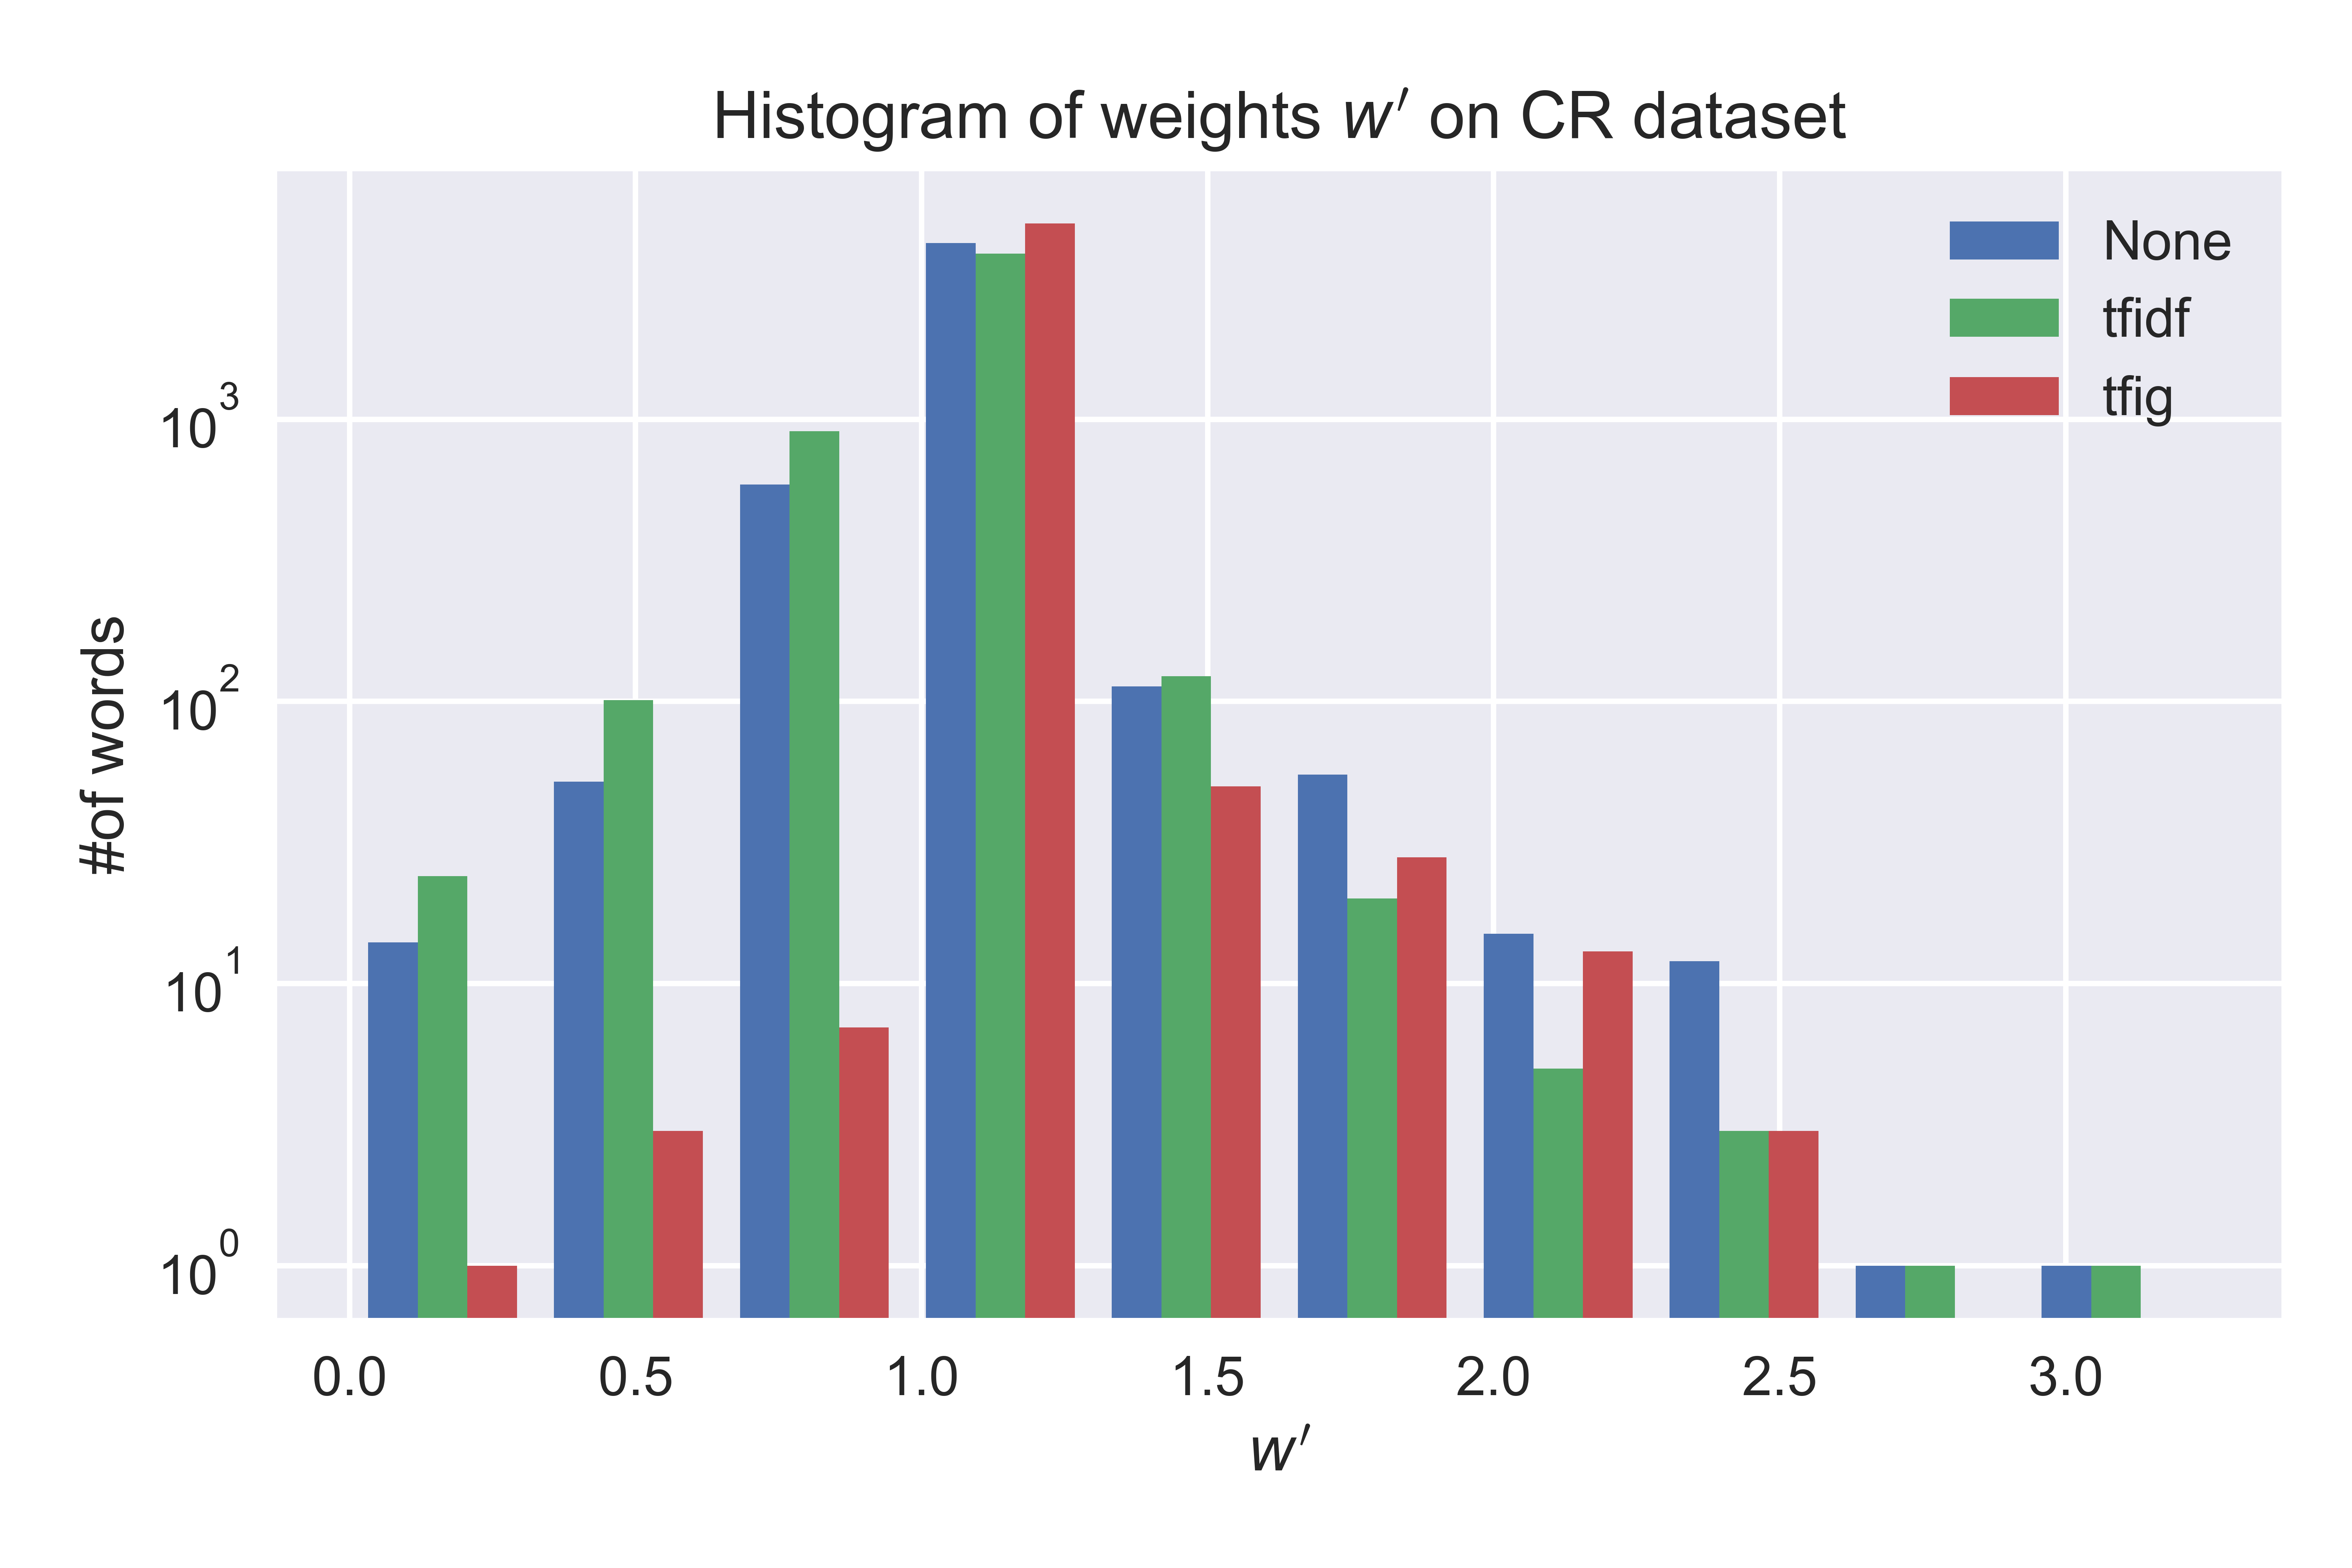
\includegraphics[width=0.7\textwidth]{images/histw_cr.png}}
    \caption[Histogram of weights $w'$ on s CR dataset]{Histogram of weights $w'$ on s CR dataset}
    \label{obr:hist:cr}
    \end{figure}

    \begin{figure}
    \centerline{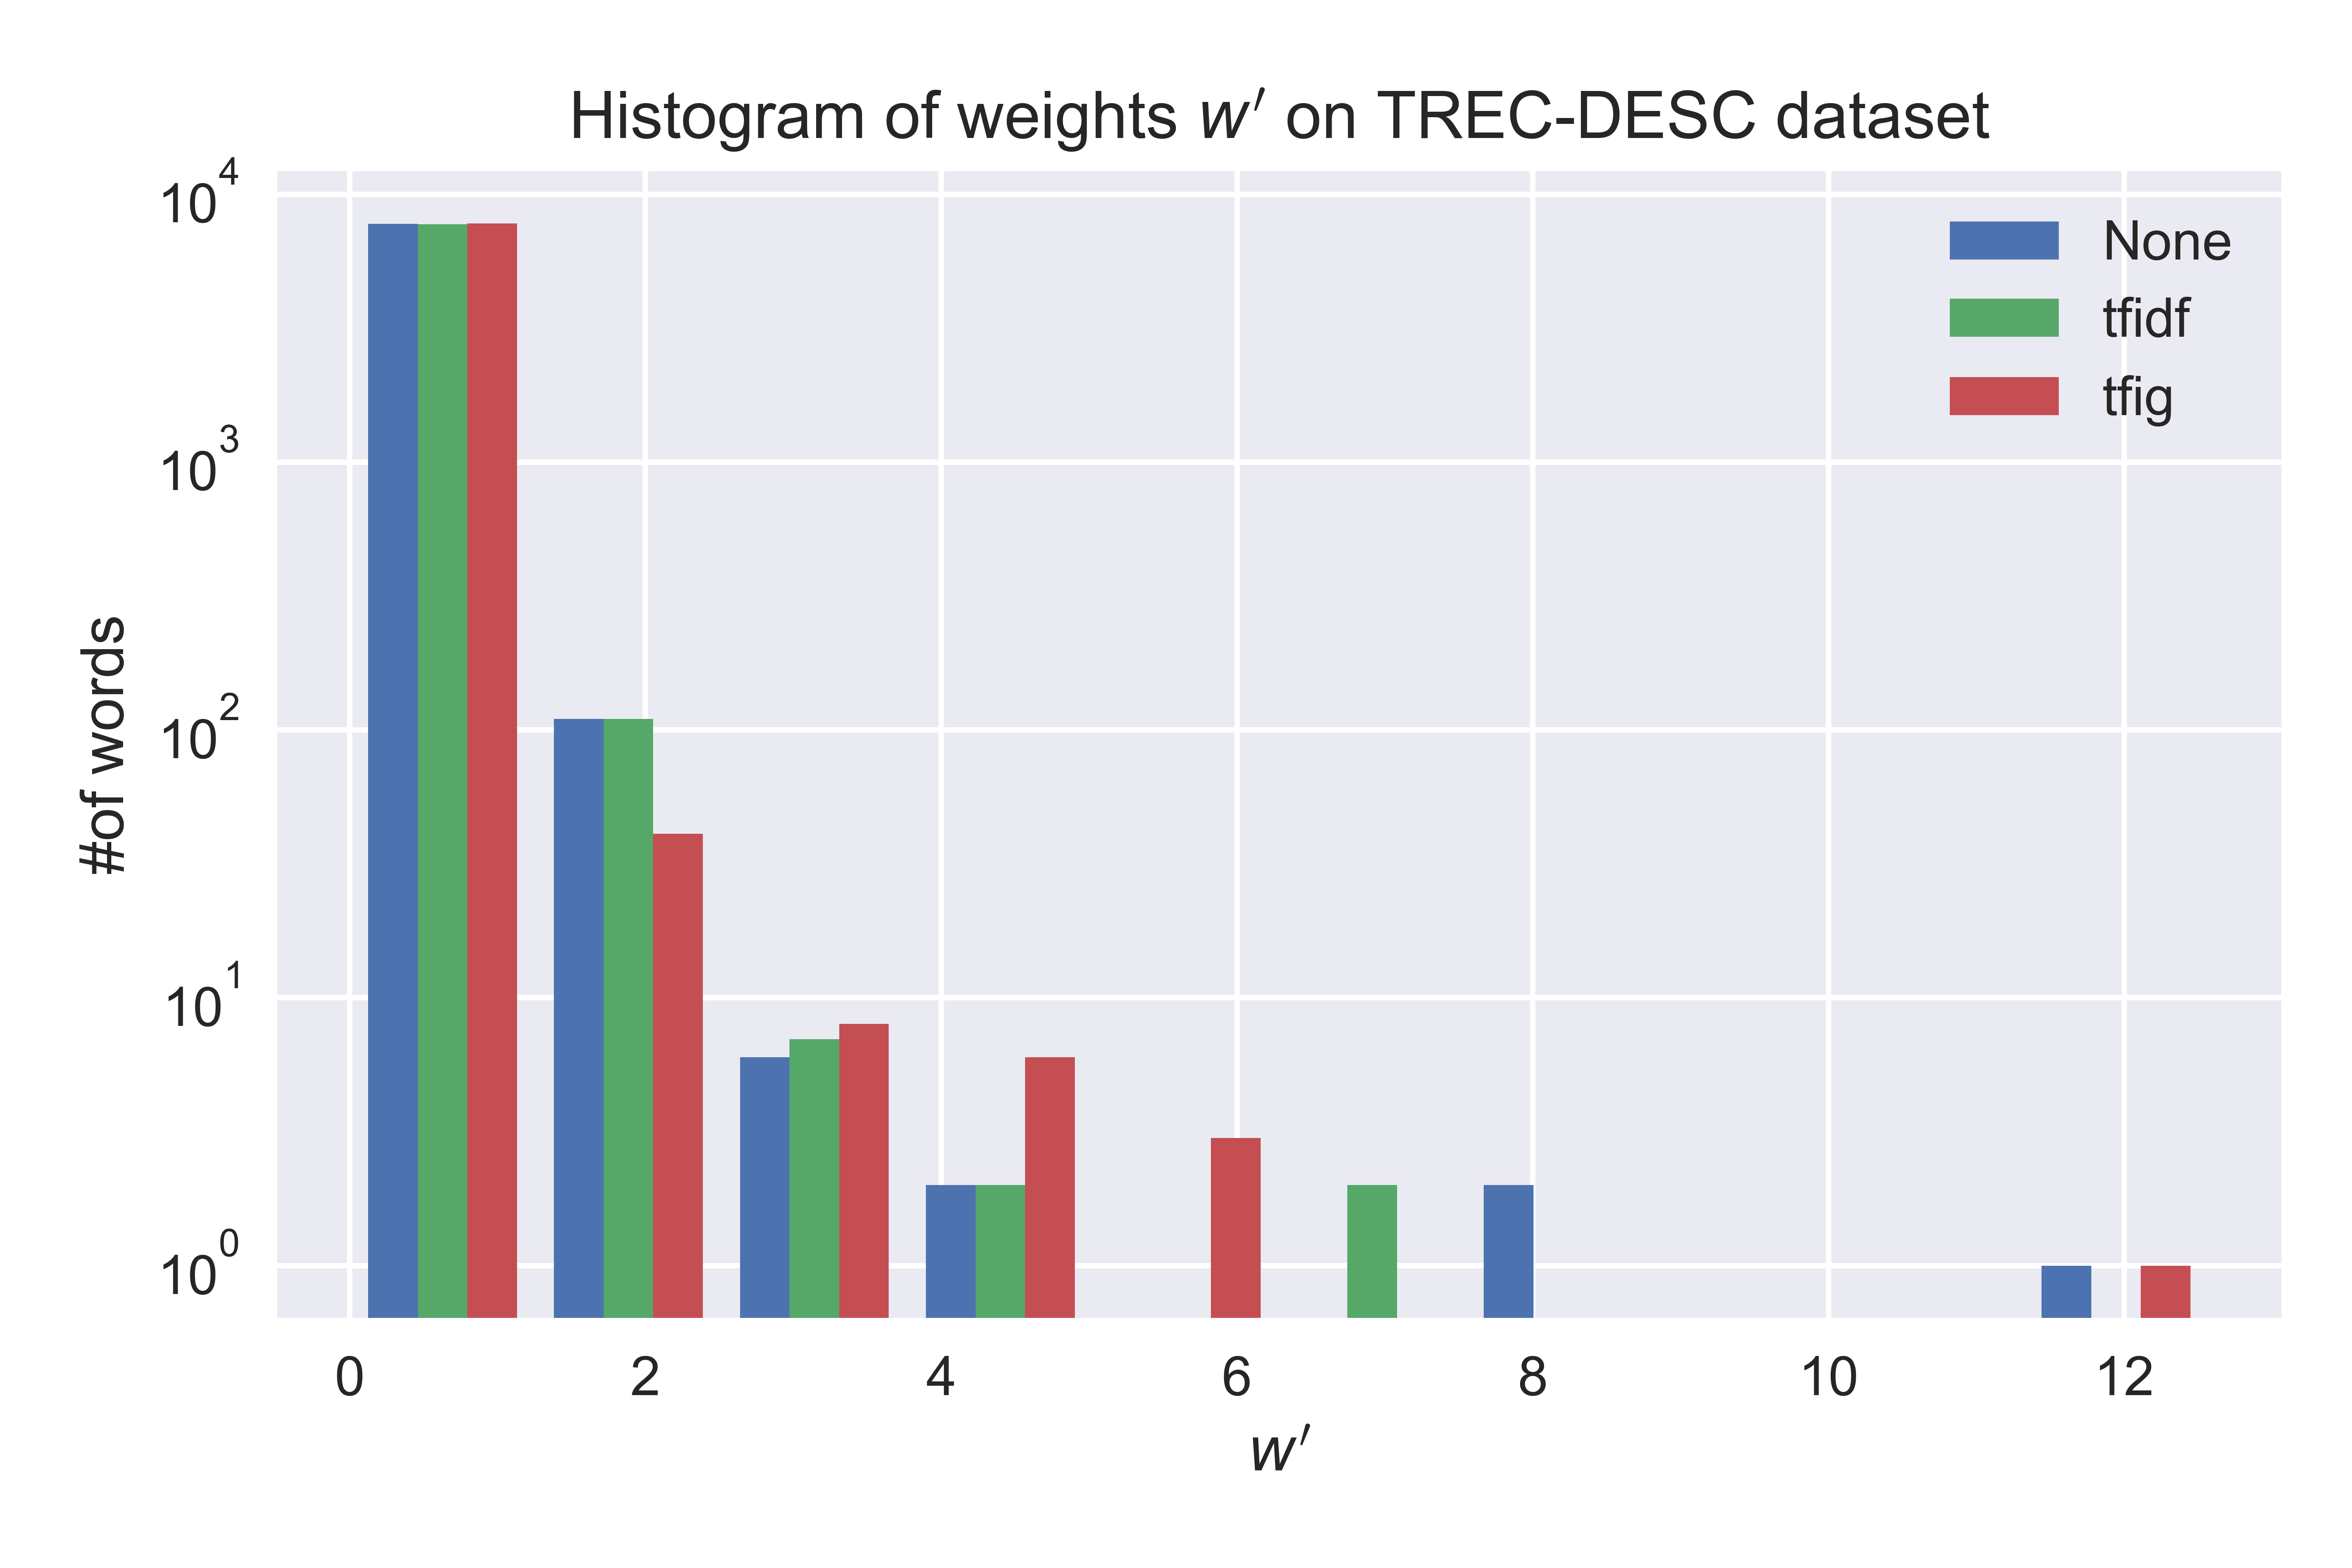
\includegraphics[width=0.7\textwidth]{images/histw_desc.png}}
    \caption[Histogram of weights $w'$ on s TREC-DESC dataset]{Histogram of weights $w'$ on s TREC-DESC dataset}
    \label{obr:hist:desc}
    \end{figure}

    On graph~\ref{obr:hist:cr} we see that \texttt{tfidf} and \texttt{None} schemes generally overweight on the CR dataset.
    We see \texttt{tfig} produces low values of $w'$ less times than \texttt{None} and \texttt{tfidf}.
    
    \subsubsection{Possible further directions for analysis}
    
    There is a number of other interesting analysis that can be performed on parameters $w'$ and may be subject to future work.
    
    We think that the most interesting, and possibly the hardest task, would be to find the analytic formula for such weighted scheme that incorporates the learned parameters $w'$. 
    This could lead to a design of a new supervised weighting scheme with better performance than current ones.
    
    To learn such analytic formula, we recommend to use symbolic regression.
